%%%%%%%%%%%%%%%%%%%%%%%%%%%%%%%%%%%%%%%%%
% University Assignment Title Page 
% LaTeX Template
% Version 1.0 (27/12/12)
%
% This template has been downloaded from:
% http://www.LaTeXTemplates.com
%
% Original author:
% WikiBooks (http://en.wikibooks.org/wiki/LaTeX/Title_Creation)
%
% License:
% CC BY-NC-SA 3.0 (http://creativecommons.org/licenses/by-nc-sa/3.0/)
% 
% Instructions for using this template:
% This title page is capable of being compiled as is. This is not useful for 
% including it in another document. To do this, you have two options: 
%
% 1) Copy/paste everything between \begin{document} and \end{document} 
% starting at \begin{titlepage} and paste this into another LaTeX file where you 
% want your title page.
% OR
% 2) Remove everything outside the \begin{titlepage} and \end{titlepage} and 
% move this file to the same directory as the LaTeX file you wish to add it to. 
% Then add \input{./title_page_1.tex} to your LaTeX file where you want your
% title page.
%
%%%%%%%%%%%%%%%%%%%%%%%%%%%%%%%%%%%%%%%%%
%\title{Title page with logo}
%----------------------------------------------------------------------------------------
%	PACKAGES AND OTHER DOCUMENT CONFIGURATIONS
%----------------------------------------------------------------------------------------

\documentclass[12pt]{article}
\usepackage[english]{babel}
\usepackage[utf8x]{inputenc}
\usepackage{amsmath}
\usepackage{graphicx}
\usepackage{subfig}
\usepackage[colorinlistoftodos]{todonotes}
\usepackage[font={small,it}]{caption}
%% Image optimons
\graphicspath{{Images/}}
\usepackage{float}

\begin{document}

\begin{titlepage}

\newcommand{\HRule}{\rule{\linewidth}{0.5mm}} % Defines a new command for the horizontal lines, change thickness here

\center % Center everything on the page
 
%----------------------------------------------------------------------------------------
%	HEADING SECTIONS
%----------------------------------------------------------------------------------------

\textsc{\LARGE Università degli studi di Milano-Bicocca}\\[1cm] % Name of your university/college
\textsc{\Large Advanced Machine Learning }\\[0.3cm] % Major heading such as course name
\textsc{\large Final Project}\\[0.1cm] % Minor heading such as course title

%----------------------------------------------------------------------------------------
%	TITLE SECTION
%----------------------------------------------------------------------------------------

\HRule \\[0.4cm]
{ \huge \bfseries Fruits 360 Challange}\\[0.4cm] % Title of your document
\HRule \\[1.5cm]
 
%----------------------------------------------------------------------------------------
%	AUTHOR SECTION
%----------------------------------------------------------------------------------------

\large
\emph{Authors:}\\
Davide Toniolo - 800458 - d.toniolo2@campus.unimib.it\\   % Your name
Omar Ghetti - 793181 - o.ghetti@campus.unimib.it   \\[1cm] % Your name

% If you don't want a supervisor, uncomment the two lines below and remove the section above
%\Large \emph{Author:}\\
%John \textsc{Smith}\\[3cm] % Your name

%----------------------------------------------------------------------------------------
%	DATE SECTION
%----------------------------------------------------------------------------------------

{\large \today}\\[2cm] % Date, change the \today to a set date if you want to be precise

%----------------------------------------------------------------------------------------
%	LOGO SECTION
%----------------------------------------------------------------------------------------


\includegraphics{logo.png}\\[1cm] % Include a department/university logo - this will require the graphicx package
 
%----------------------------------------------------------------------------------------

\vfill % Fill the rest of the page with whitespace

\end{titlepage}


\begin{abstract}
The Fruits 360 is an image recognition challenge from Kaggle. In this article a few CNN solution proposals are presented, some of which were obtained through transfer learning, while others were built from scratch. From the initial batch of models, the most promising ones were selected and went through Hyperparameter Optimization to further improve their performance.
\end{abstract}

\section{Introduction}
The field of Computer Vision is a subset of the research on (\textit{narrow} or \textit{weak}) Artificial Intelligence and its goal is that of building machines capable of perception of visual stimuli and perform tasks as image classification, object recognition, image segmentation, image description, reconstruction of trajectories, etc... .

In the past decade, CV saw a few important breakthroughs and increased interest and it's one of the most rapidly evolving domains of study in the Artificial Intelligence and Computer Science communities.

The reason for the increased popularity of CV is a breakthrough presented at the ImageNet challenge in 2012 (ref \cite{ImageNet2012}). In that year for the first time the challenge was won by a neural network, called AlexNet \cite{NIPS2012_4824}. This ANN significantly outerformed all the competitors and begun a new wave of interest in CNN, which since them have been applied to an increasing number of tasks with considerable success.

The main driver of this breakthrough is the use of Convolutional Neural Networks (CNNs for short), of which AlexNet is regarded as the first really effective one. CNNs rely on the usage of a mathematical operation called convolution\footnote{The correct name is \textit{cross-correlation} (ref \cite[[Chapter~9]{DeepLearningBook}), however the difference between the two definitions often isn't relevant in the usage of CNNs.}, which encodes in the network the translationally invariant properties of many vision dataset. A convolutional layer therefore encodes a known property of the dataset in the model itself, vastly reducing the search space and therefore greatly improving training times.

CNNs have been known for many years before AlexNet, but it was the first really successful application of them, thanks to the novel way in which it combined structure, activations, and other factors. CNNs have become the go-to approach for complex CV tasks, and since then all the ImageNet competitions have been won by a convolutional neural network.

The goal of this article is to solve an image classification task. Both custom and pre-built models are used, evaluated and discussed. 


\section{Datasets}
The corresponding dataset consists of 80 000 images of 120 varieties of fruits. All the images have a resolution of 100x100 pixels and show the subject centrered and with a white background, as seen in the examples in figure \ref{img:examples}. The dataset was published already separated in train and test set.

\begin{figure}[H]
	\centering
	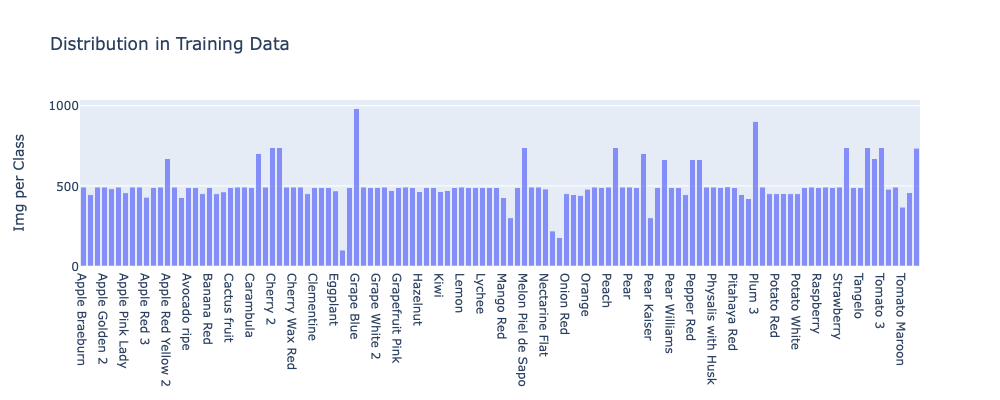
\includegraphics[width=\textwidth]{Distribution.png}
	\caption{Distribuition of training data: classes are well balanced}
	\label{img:tdd}
\end{figure}

\begin{figure}[H]
	\centering
	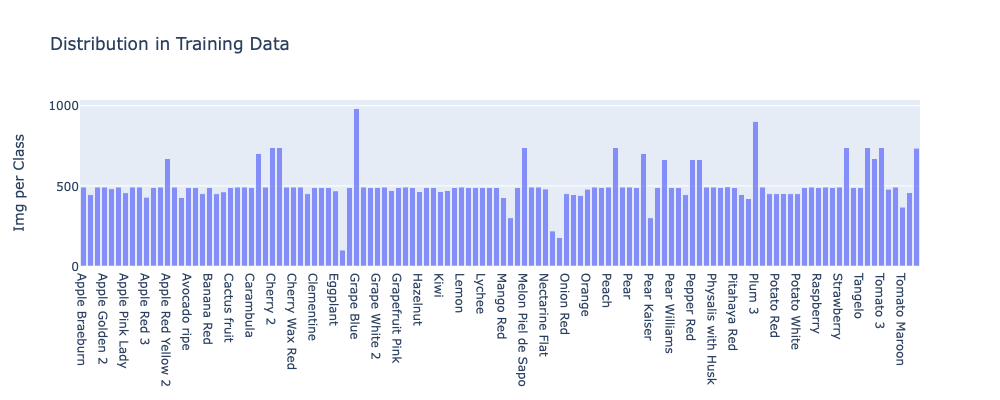
\includegraphics[width=\textwidth]{Distribution.png}
	\caption{Distribuition of test data:}
	\label{img:distribuition_of_test_data}
\end{figure}

The class frequency is balanced in both the train and test set. The balance is sufficiently good to make the accuracy a valid metric. Still, given the different classes, the confusion matrix needs to be taken into account: it is possible for the model to do exceptionally well on some classes and bad on others, even if the balanced data makes this unlikely.

\begin{figure}[H]
	\centering
	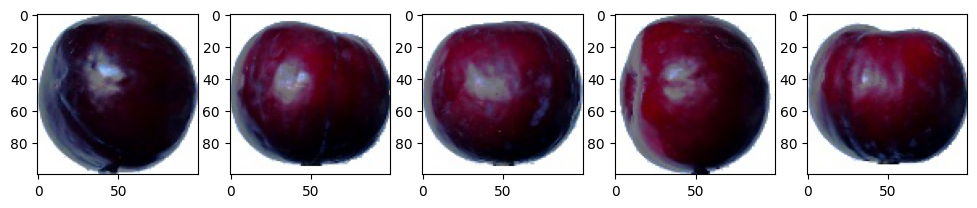
\includegraphics[width=\textwidth]{imgExample.png}
	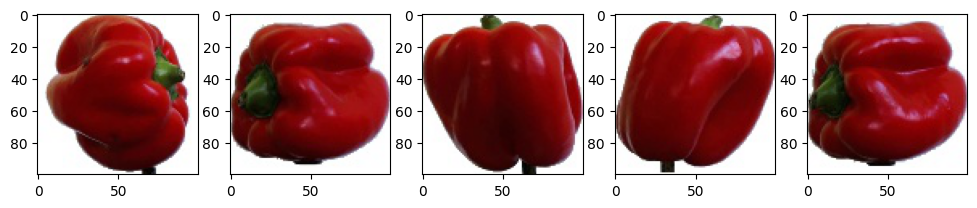
\includegraphics[width=\textwidth]{imgExample2.png}
	\caption{Samples of some images in the dataset}
	\label{img:examples}
\end{figure}

\section{The Methodological Approach}
\subsection{Transfer Learning} \label{sub:transferlarning}
The models to use for transfer learning are chosen among the top performers in the ImageNet challenge \cite{ILSVRC15} for a given year. They were selected according to two criteria:
\begin{itemize}
	\item variety of theoretical approach. The models are the result of papers which introduce new theoretical ideas. We tried to represent them all while maintaining a good variety at the same time. 
	\item ease of use in the Deep Learning Framework of choice (Tensorflow). Some of the state.of-the-art efforts are not yet available in this library (e.g. AlexNet). Their use would have required a lengthy conversion process from other frameworks, like Caffè, Theano or PyTorch.
\end{itemize}

The selected solutions are:
\begin{itemize}
	\item VGG16, proposed by K. Simonyan and A. Zisserman from the Univeristy of Oxford, is one of the famous models submitted to the ILSVRC-2014 Challenge. This network makes an improvement over AlexNet by replacing large kernel-sized filters with multiple 3x3 kernel-sized filters one after another.
	\item Inception v3 \cite{DBLP:journals/corr/SzegedyVISW15}. The original Inception \cite{DBLP:journals/corr/SzegedyLJSRAEVR14} introduces the network-in-network approach. We chose the 3rd version because it was presented as an improvement with respect to the 1st.
	\item ResNet50 \cite{DBLP:journals/corr/HeZRS15}, which is the first to make an extensive use of skip connections.
\end{itemize}
%\begin{figure}[H]
%	\centering
%	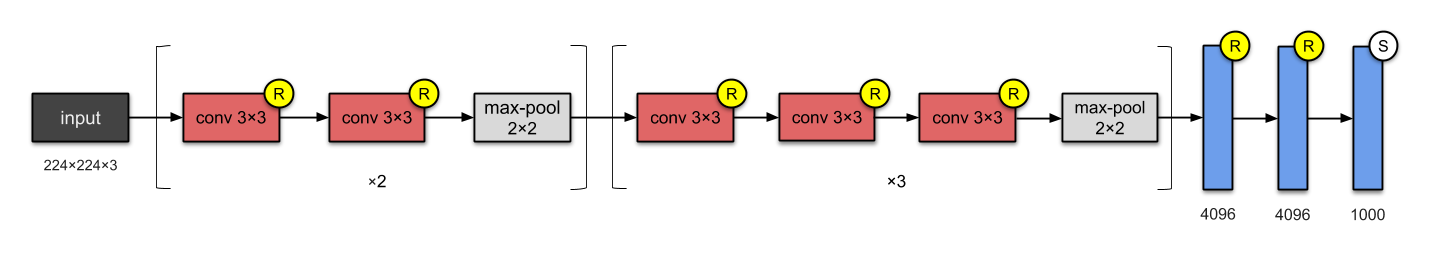
\includegraphics[width=\textwidth]{VGG16.png}
%	\caption{High level structure of the VGG-16 neural network. The overall depth (excluding the non-trainable max pooling operatorions) is of 16 layers - exactly twice than AlexNet. This net as a large number of parameters, $\sim$ 138M. After VGG-16, many efforts of the CNN research community were aimed at finding architectures with the same performance and a lower memory footprint.
%	\label{img:vgg16}
%\end{figure}

%\begin{figure}[H]
%	\centering
%	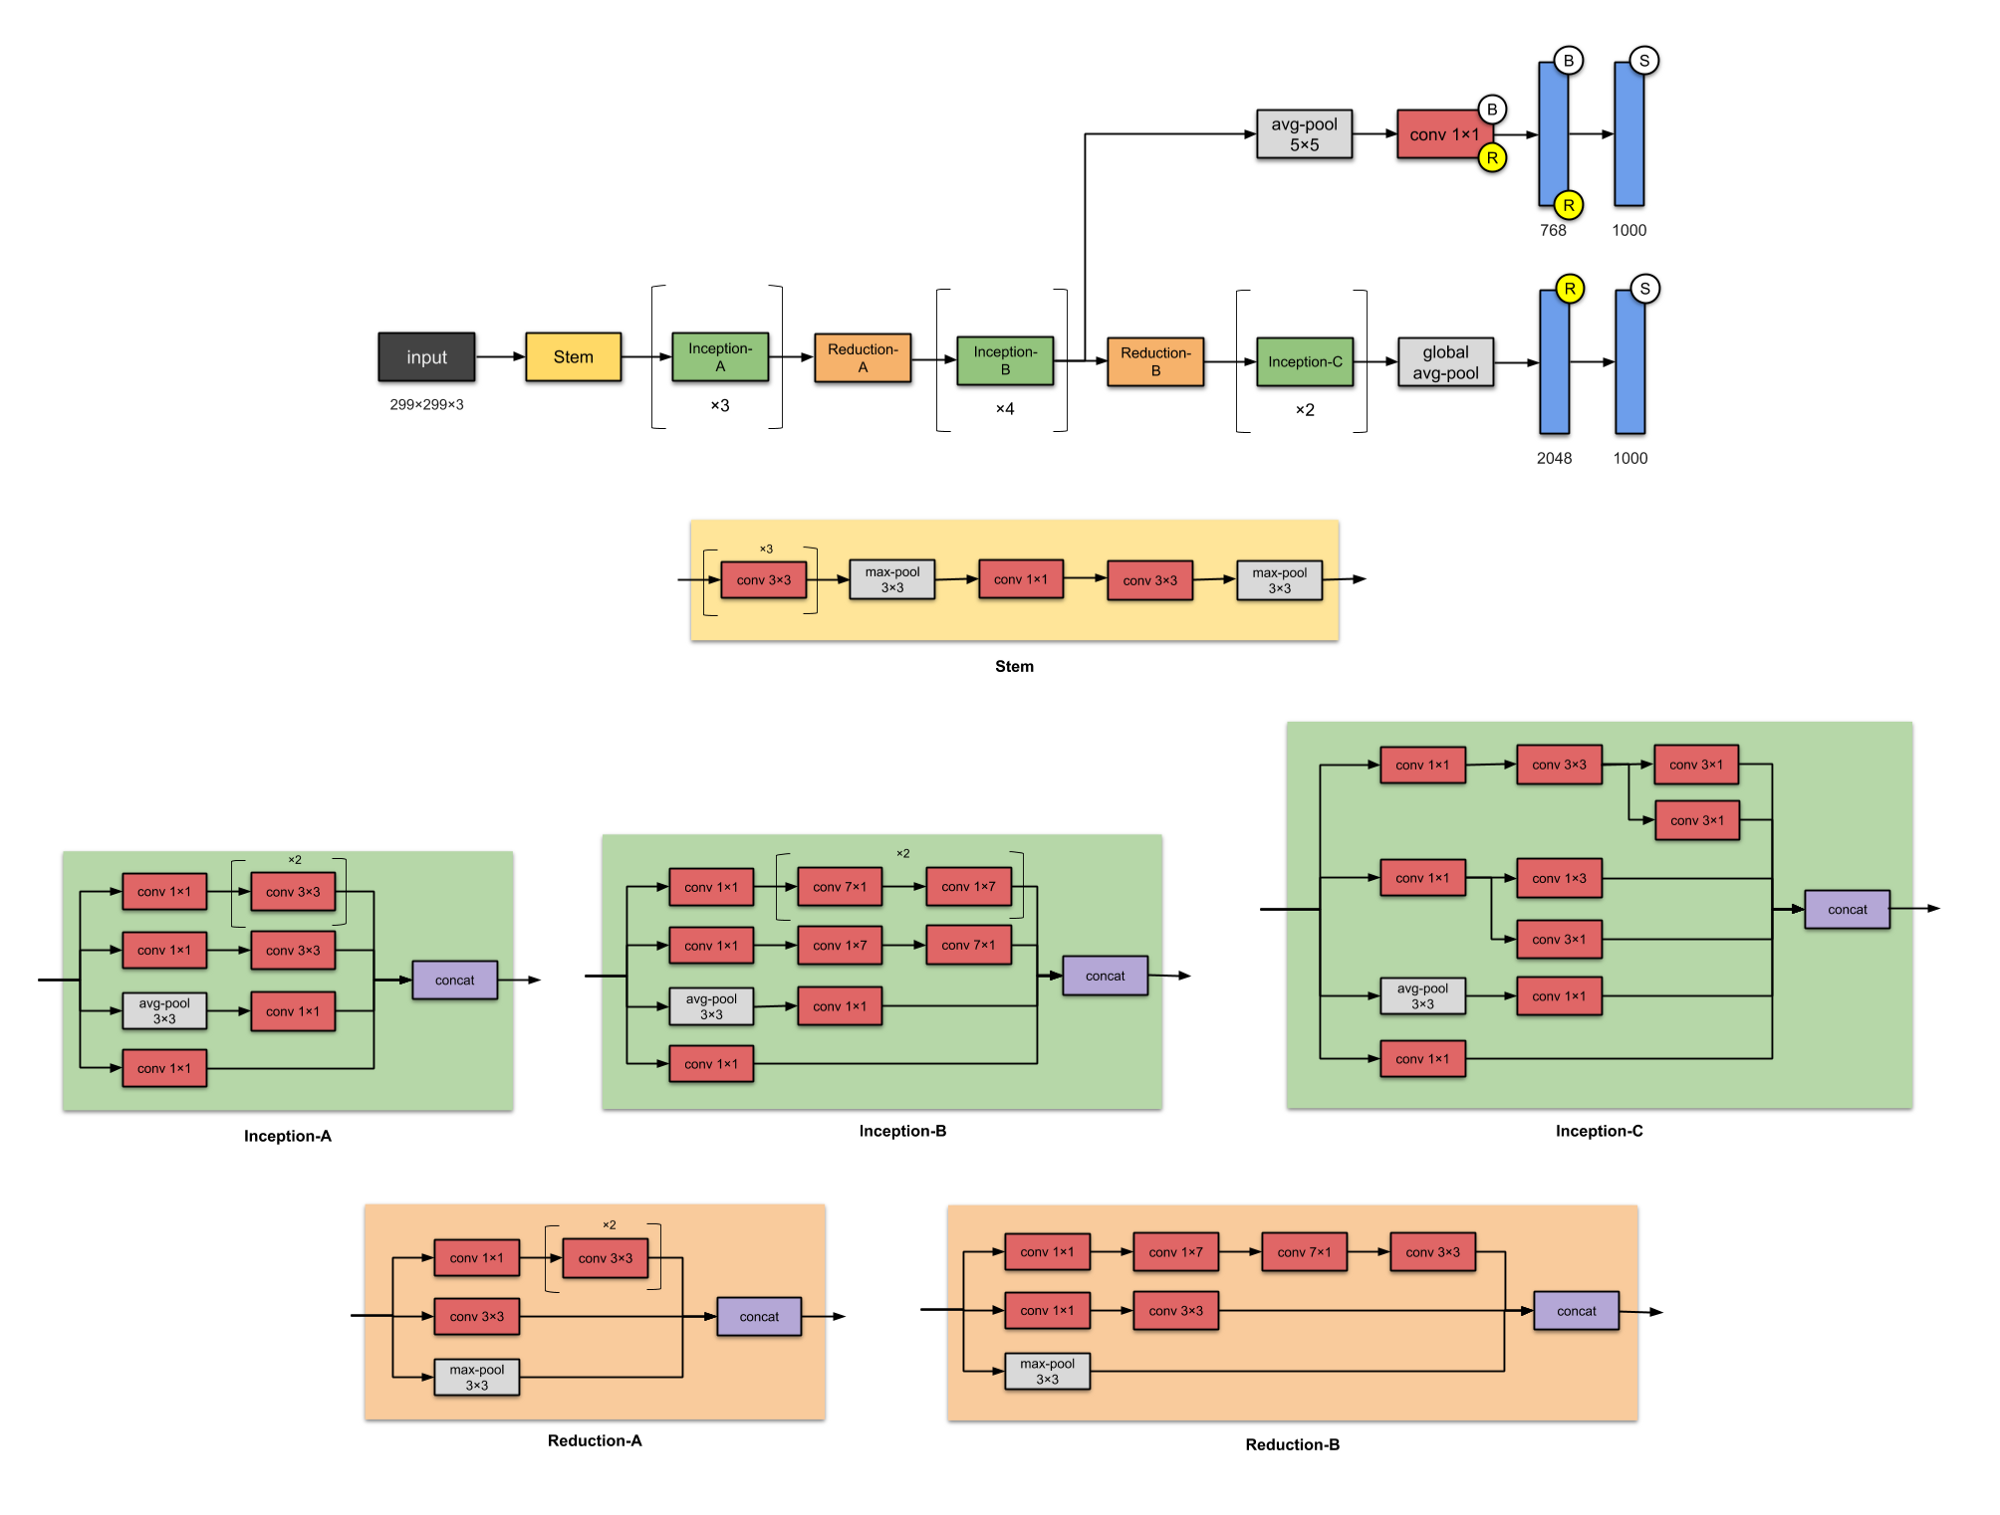
\includegraphics[width=\textwidth]{Inception v3.png}
%	\caption{Structure of Inception v3. Each module is a small neural network. Due to the way the so-called ``''Inception modules``'' are designed, they can achieve a great representational capacity with a small number of parameters. \\
% auxiliary branch is used to better propagate back the gradients during training time, and is discarded during inference.}
%	\label{img:inception}
%\end{figure}

%\begin{figure}[h!]
%	\centering
%	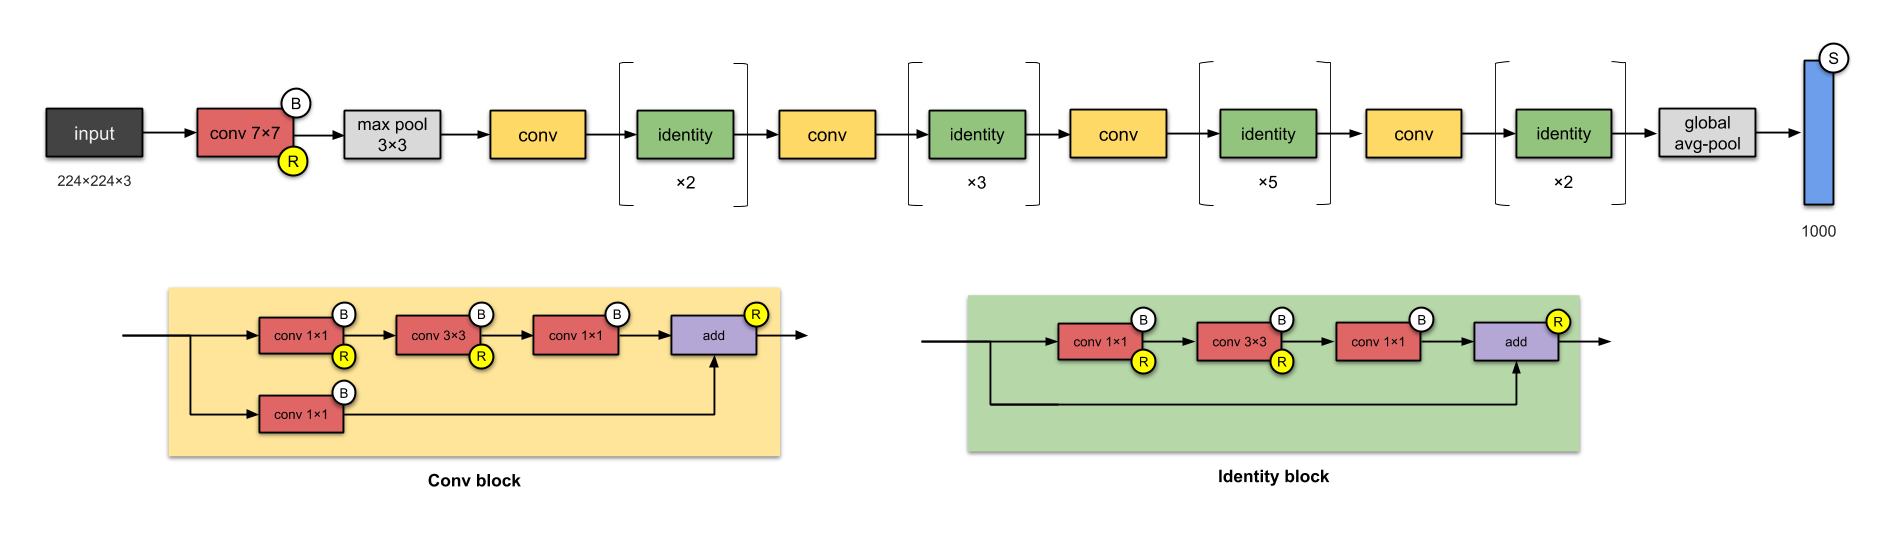
\includegraphics[width=\textwidth]{ResNet50.png}
%	\caption{The ResNet50 convolutional ANN. It relies on the network-in-network idea introduced by the Google Brain team with the Inception networks, but also explores the use of skip connections for better back propagation. Skip connections are only used inside each module, but later efforts have also direct paths between different cells.}
%	\label{img:inception}
%\end{figure}

With the sole exception of the final classification layer, all the others were kept and used the weights published by the researchers. We trained only the new classification layer first, and then all the network. We can then analyse how well these model transfer to the Fruits 360 dataset, and how much there is to gain when performing the full optimisation.
These neural networks have been imported and stripped of their classification layers, which have been replaced by smaller ones for the task at hand.

Illustration of the structures of these networks can be found inside the Extras directory included with the pdf file of this report. They are courtesy of Raimi Karim, see the excellent, albeit informal article \cite{IllustratedCNN}.

\subsection{Custom Model}
A simple custom model has been built, aiming at a small, but functional network. A limited number of layers and parameters was deemed to be important for two reasons:
\begin{itemize}
	\item training even a simple CNN from scratch requires a considerable amount of time and resources, and
	\item as the network gets more complicated the number of possible configurations grows exponentially, making it harder to make principled choices and explore different solutions.
\end{itemize}

The selected configuration is the following:

\begin{table}[h!]
	\centering
	\begin{tabular}{| l | c | c | c | c | c |}
		\hline
		Layer & Filters & \multicolumn{1}{|p{2cm}|}{\centering Kernel or \\ Pool Size} & Stride & Padding & Activation\\
		\hline
		 Convolutional 1 & 128 &  3x3 & 1x1 & ``same'' & rectifier \\
		 Max Pooling && 2x2 & 1x1&&\\
		 Convolutional 1 & 64 &  3x3 & 1x1 & ``same'' & rectifier \\
		 Global Max Pooling &&&&& \\
		 - & Units & &&& \\
		 Fully Connected, classification & 120 & && &softmax\\
		 \hline
	\end{tabular}
	\caption{Structure of the custom model. It is very limited depth and width compared to  those discussed previously.}
	\label{tbl:custom_model_structure}
\end{table}


\subsection{Hyperparameter Tuning}
For every model described in section \ref{sub:transferlarning} a procedure of Hyperparameter Tuning as been implemented to maximise the performances of the models trying different combinations of hyperparameters. The Learning Rate $\epsilon$, the dropout rate $\mu$ and (when relevant) the weight $\alpha$ of the $L^2$ regularisation on the classification layer.

The procedure has been implemented using two different libraries:
\begin{itemize}
	\item Scikit-Optimize, or skopt, is a simple and efficient library to minimise (very) expensive black box functions. It implements several methods for sequential model-based optimisation and has a few visualisation utilities.
	\item Keras Tuner, a library that helps you pick the optimal set f hyperparameters for your Tensorflow program.
\end{itemize}

The two libraries provide all the most common algorithms for AutoML, such as Bayesian Optimisation, Random Search, etc... . Random Search was used for VGG-16 and ResNet50, while Inception v3 and the custom model went through a Random Forest HPO. Each model was trained for a number of epochs variable between 2 and 10, for a total of 10 different hyperparameter configurations, and checkpoints were implemented to save only the best results and quit the training process if the metrics weren't good enough, or they were not improving. After finding the best hyperparameters, every model went through a new retrain with the optimized parameters, to ensure the best performances possibile.

\subsection{Training Procedure}
The training set was further split into a training and a validation set. The latter was used for the HPO and once the best hyperparameter configuration had been found, the corresponding model was retrained from scratch using both the training and the validation using the newly found hyperparameters.

The data was fed to the model by Keras genererators that performed tasks of data augmentation by rotating, flipping and scaling the images.


\section{Results and Evaluation}
\subsection{A Word on Notation}
For the shake of brevity, from now on the learning rate, the $L^2$ regularisation weight and the dropout rate will be referred to as, respectively, $\epsilon$, $\alpha$ and $\mu$.

\subsection{VGG16}
VGG16 was the best performer regarding pure training accuracy in the first runs, but a problem with noise in validation accuracy and loss was clear from the beginning. Data augmentation was applied to the images and the preprocesssing function was used on the generators to prepare the images. the top layer applied to the existing network was composed by a Flatten layer, a Dense layer with 1024 units and a Dropout layer with 0.6 of Dropout Rate. all of this followed by a Dense classificator with softmax activation function. After HPO, Dropout Rate was lowered from 0.6 to 0.2 while learning rate moved up from 0.00001 to 0.0001. After just 4 epochs, retrain with optimized parameters stopped because there were no more improvements to see in the next steps.
\begin{table}[H]
	\centering
    \addtolength{\leftskip} {-2cm} % increase (absolute) value if needed
    \addtolength{\rightskip}{-2cm}
	\begin{tabular}{ |c|c|c|c|c| }
		\hline
		Train Acc. (\%)& Val. Acc. (\%) & Train Loss (nats) & Val. Loss (nats) & Test Acc (\%)\\
		\hline
		98.66 & 97.46 & 0.0762 & 0.0993 & 98.00\\
		\hline
	\end{tabular}
	\caption{Results for VGG-16.}
	\label{table:vgg16_res}
\end{table}
\begin{figure}[H]
\centering
\subfloat[accuracy]{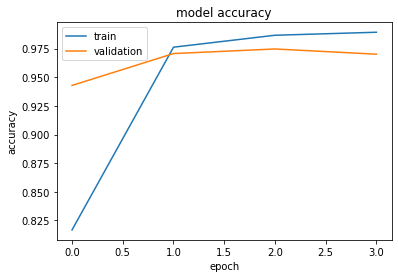
\includegraphics[width=0.4\textwidth]{VGG16_HPOaccuracy.png}}
\hfill
\subfloat[loss]{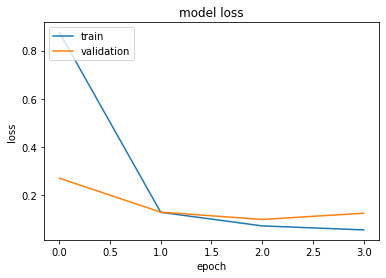
\includegraphics[width=0.4\textwidth]{VGG16_HPOLoss.png}}
\caption{Plots for Accuracy and Loss for VGG16} 
\end{figure}

\subsection{ResNet50}
ResNet50 was initially the worst performer between the three networks tested. After the application of the right preprocessing function and some data augmentation to the images, a top layer composed by a Flatten layer, one Dense layer with 128 units and relu activation function, a Dropout layer with 0.6 rate and a Dense classifier with softmax activation function, was added to the network. After 10 epochs of training, result were good on the training side but really bad on validation side, reporting a clear overfitting problem. After HPO, Dropout Rate was lowered from 0.6 to 0.3 and Learning Rate was lowered from 0.001 to 0.00001, and the new retrain showed optimal result in both testing and validation after just 6 epochs.
\begin{table}
	\centering
	\addtolength{\leftskip} {-2cm} % increase (absolute) value if needed
	\addtolength{\rightskip}{-2cm}
	\begin{tabular}{ |c|c|c|c|c| }
		\hline
		Train Acc.(\%) & Val. Acc.(\%) & Train Loss (nats) & Val. Loss (nats) & Test Acc (\%)\\
		\hline
		99.42 & 98.40 & 0.0413 & 0.0658 & 98.60\\
		\hline
	\end{tabular}
	\caption{Results for ResNet50}
	\label{table:resnet50_res}
\end{table}

\begin{figure}[H]
\centering
\subfloat[accuracy]{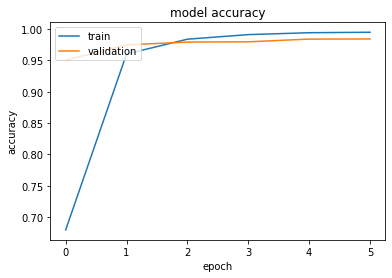
\includegraphics[width=0.4\textwidth]{renset50_hpoAccuracy.png}}
\hfill
\subfloat[loss]{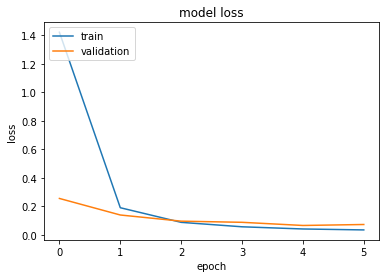
\includegraphics[width=0.4\textwidth]{resnet50_HPOloss.png}}
\caption{Plots for Accuracy and Loss for ResNet50}
\end{figure}

\subsection{Inception v3}
The two final classification layers where stripped away and were replaced with only one fully connected layer with softmax activation. Only one layer was used, because early experiments with both one and two FC layers suggested that the latter was prone to overfitting and didn't achieve a much higher performance.

The same early experiments showed that, even with only one FC layer, this Inception network struggled to match its training performance on the validation set. In order to improve generalisation, a few regularisation strategies were evaluated: $L^1$ and/or $L^2$ penalties on the last layer; and dropout layer right after the global average polling.

The $L^1$ regularization showed poor results on the training set performance, even with low values of $\alpha$. The other two were more promising and were included in the HPO. We were cautious in introducing the Dropout regularisation strategy because the network includes a great number of batch normalisation layers, which are deemed to work poorly with dropout (ref ??).

The Hyperparameter Optimization process selected an $\alpha$ and a dropout rate that where orders of magnitude lower than what commonly employed, suggesting that they were not necessary. Specifically, the dropout rate is $\sim 10^{-3}$, while $\alpha\sim 6\cdot 10^{-9}$, compared to what are commonly considered the industry ``safe'' standards of $0.1$ or $0.8$ for the dropout and $10^{-3}$ for $\alpha$\footnote{These values are, for example, the default values in Tensorflow. They aren't absolutes truths and many authors suggest not trusting them, but still, differences of many orders of magnitude are relevant.}.

The learning rate is very similar to the usual default for Adam. However, this hyperparameter is regarded as one of the most sensible and relevant (ref ?? and ??), and a the small difference might be significant. So, as a final configuration, we suggest removing the dropout and the $L^2$ regularisation, and keep only the learning rate from the HPO.

The model trained with the HPO parameters showed improved performance, but not greatly so. We regard the improvement to the result of only the better $\epsilon$ and suggest that the small dropout and $L^2$ regularizations have no significant impact.
\begin{table}[H]
	\center
	\begin{tabular}{ |c|c|c|c|c| }
		\hline
		Train Acc. (\%) & Test Acc.(\%)  & Train Loss (nats) & Test.Loss (nats) \\
		\hline
		94.41 & 89.26 & 0.0413 & 0.3395\\
		\hline
	\end{tabular}
	\caption{Results for Inception v3}
	\label{table:inc3_res}
\end{table}
\begin{figure}[H]
	\centering
	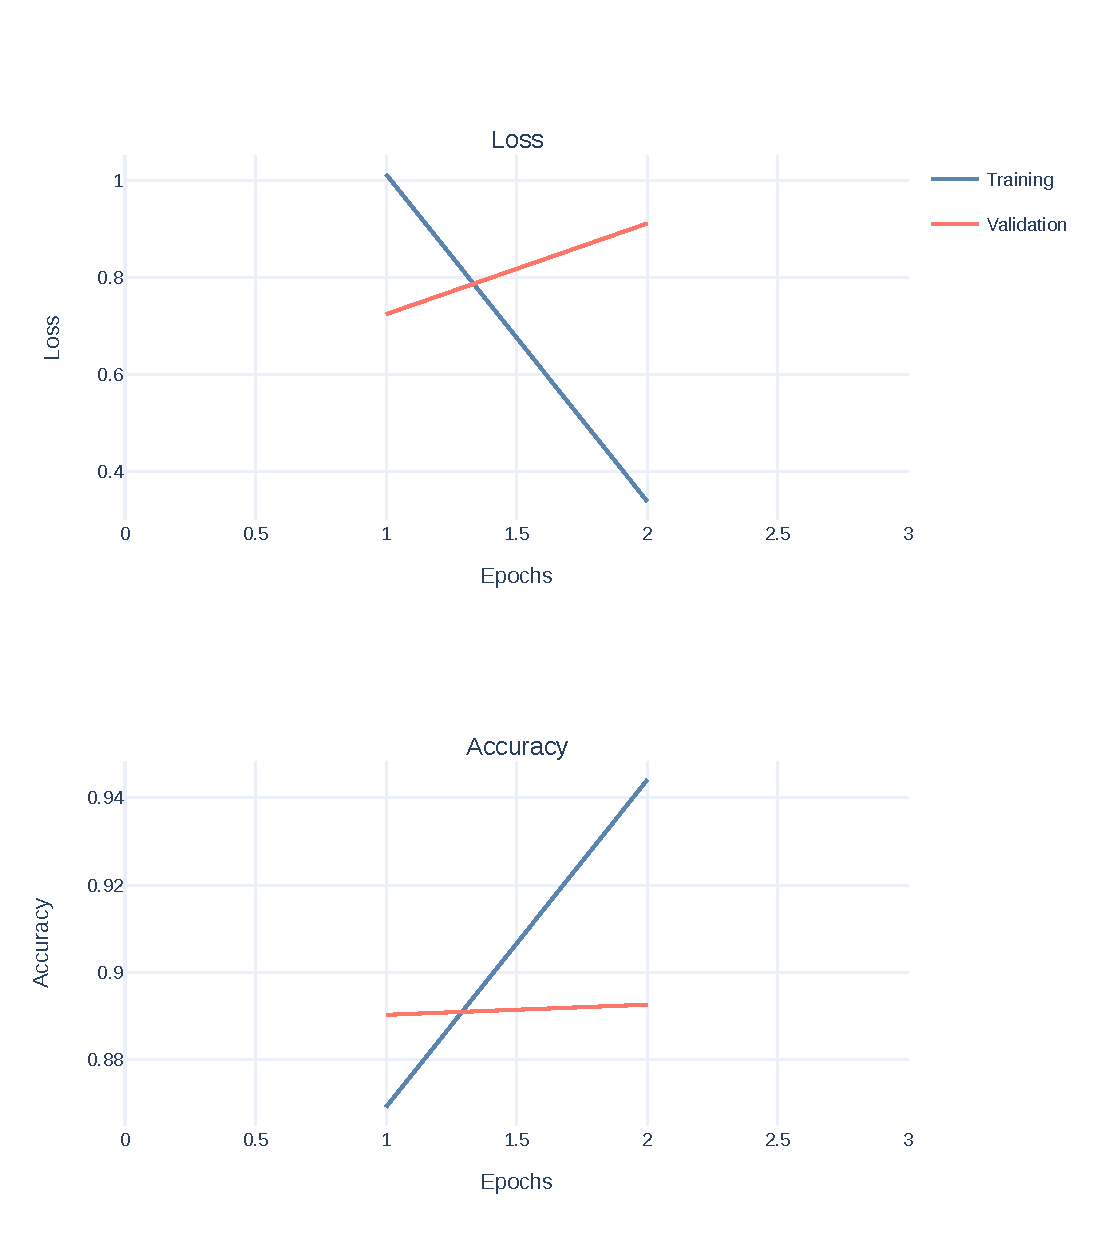
\includegraphics[width=0.9\textwidth]{Inception v3 After HPO 2020-06-16 09_42_52.491141.pdf}
	\caption{Plots for Accuracy and Loss for Inception v3. Due to the limited number of epochs, the plots are minimal. Please note that these two refer to the training on both the training and the  validation sets, so that the ``validation'' lines refer to the test set.}
	\label{fig:inv3_results}
\end{figure}

\subsection{Custom Model}
The custom model showed promising results from the beginning, outperforming the models obtained from transfer learning. For example, an early exploratory training showed great performances with no regularisation other than the data augmentation and the early stopping:
\begin{table}[h!]
	\centering
	\begin{tabular}{ |c|c|c|c|c| }
		\hline
		Train Acc. (\%) & Val. Acc. (\%) & Train Loss (nats) & Val. Loss (nats)\\
		\hline
		98.08 & 92.67 & 0.0561 & 0.3273\\
		\hline
	\end{tabular}
	\caption{Performances of the custom model at the beginning of the exploratory analysis.}
	\label{tbl:custom_model_performance_beginning}
\end{table}

At this stage, we had no way to tell wether we had hit a lucky hyperparameters configuration or if this model had more capacity than the others. However, even after the HPO the other models failed to match these results, so that we can say that this model's architecture is likely to be more effective for the task at hand.

The HPO process reserved a surprise for this model: what was deemed to be the best configuration turned out to have very poor performance (training loss $>$ 100) when used for retraining the network. We suggest that, by chance, this configuration had overfit the validation set and was chosen because only one metric was tracked during the HPO.

None of the other configurations surpassed the one with the default hyperparameters, so that the former was used as the final one. This issue is part of a broader set of problems that arose with the usage of skopt, which are discussed in the subsection \ref{furtherimprovements}.

\section{Discussion}
All the models are able to reach over 98\% accuracy. The much smaller custom model is able to match the performance of the larger ones from the ImageNet challenge. It would be interesting to observe what the model's performance would be after an HPO.

The main reason for this lack of difference is likley to be found in the different statistical properties of the Fruits 360 dataset and that of the ImagNet challange: the task at hand is orders of magnitue simpler than the broader image recognition challenge. All the subjects have a, white uniform background and have similar features. A model that learn to distinguish color, shape and texture can presumably achieve a reasonable performance.

The ImageNet challange, on the contrary, requires a model able to deal with a great variety of backgrounds: grass, urban, inside buildings,...; and different lighting conditions. Moreover, the classes have a broder set of features: animals are present, so that it may be necessary to learn to recognize eyes, fur, ears, legs, tails, wings, etc... . But also cars (wheels, lights, ...), tools, or activities (abstract concepts).

The ability to deal with this variety isn't necessary for the Fruits 360 challenge. 



\subsection{Further Improvements}\label{furtherimprovements}
With more computational resources available, it could be possibile to perform a (manual or automatic) NAS on the custom model, in order to understand which level of depth is adeguate for this task.

To improve the efficiency of the HPO process, training curve prediction could be implemented. In this way time would not be wasted on configurations that are likely to be underperforming.

The training process of the custom model could benefit from significant speedups: an analysis of the machine usage showed that, with such a small model, the GPU is underutilized. The real bottlenecks are the data augmentation process occurring on the CPU and the constant stream of data from the hard drive.

Given that the dataset is too big to be held in memory, the generator is necessary, especially considering that we want a data augmentation process. We suggest training multiple models in parallel on the same GPU and to feed them the data from the same generator: in this way we could take full advantage of the GPU's capabilityes without requiring better hardware. However, at present, we have found no simple way to create a data pipeline flowing from the generator to multiple models without having to replicate the generator process itself (which would destroy any benefit from the parallel training).

Also, Scikit Optimize had disappointig results. While the package looked promising, it was later discovered that it suffers from a few bugs unresolved from long time unresolved . The most important of them was the inability to correctly warm start the optimization process \cite{issue1}, \cite{issue2}.

The decision to use two different HPO libraries allowed the researchers to exchange their feelings about their experiences and the perceived pros and cons of each package. A joint decision to abandon skopt and use only Keras Tuner was reached. The code was written with reusability in mind, so a migration process from one framework to the other could be fast and painless.

However, this process can't be completed in time for the deadline for this report: the HPO process is a lengthy one and all the code is run inside the free Google Colab platform. This means that during each run only a handful of configurations can be explored and after there's a cool-down period during which the computational resources are unavailable. The whole process requires a couple of days.


\section{Conclusions}
All the models showed satisfactory performance and good generalisation. It was found that the statistical properties of the dataset allow for both transfer learning and new models to be trained and applied successfully. However, the usage of solutions from the ImageNet challenge yields similar or worse performance with the addition of higher memory footprints and inference times.

Overall, smaller, ad hoc models are the most promising route for an hypothetical real world application.

The HPO process greatly improved the performance of the models transferred from ImageNet and will benefit from a re-implementation in another library for Inception and the custom model.



\bibliographystyle{IEEEtran}
\bibliography{Relazione.bib}

\end{document}